% Provenance (never printed): old seconde/premiere S material on the
% atmosphere (storms, cyclones, the energy of the water cycle) and the
% natural-hazard themes of SVT; see sources/book2/PROVENANCE.md. Tracks,
% genesis statistics and the pressure--wind relation are computed in
% figdata/grade-10/cyclones.py from IBTrACS v04r01; the surge, thunder and
% energy numbers in the same script.
\chapter{Badai dan Siklon Tropis}\label{ch:g10:storms-and-cyclones}

Suatu sore musim panas yang terik berakhir dengan badai. Langit menggelap,
embusan angin dingin menyapu jalan, sebuah kilatan menerangi awan --- dan kamu
mulai menghitung: satu, dua, tiga, \ldots{} sembilan detik kemudian guntur
bergemuruh. Badai itu berada sekitar tiga kilometer jauhnya. Satu jam lagi
badai itu akan berlalu, dan udara akan terasa sejuk dan bersih. Di atas
samudra tropis yang hangat, bahan-bahan yang sama --- udara hangat dan lembap
yang naik dan mengembun --- dapat tersusun menjadi badai dengan ukuran yang
sama sekali lain: \omterm{def:g10:storms-and-cyclones:tropical-cyclone}{siklon tropis}, yang lebarnya ratusan kilometer, bertahan
berhari-hari, dan membawa angin yang cukup kuat untuk merobohkan hutan serta
kenaikan muka laut yang membanjiri seluruh pesisir. Bab ini membahas \omterm{def:g10:storms-and-cyclones:thunderstorm}{badai
guntur}, \omterm{def:g10:storms-and-cyclones:tornado}{tornado}, dan \omterm{def:g10:storms-and-cyclones:tropical-cyclone}{siklon tropis}, serta asal energinya.

\begin{safety}
Jika kamu dapat mendengar guntur, \omterm{def:g10:storms-and-cyclones:lightning}{petir} dapat menjangkaumu. Masuklah ke dalam
bangunan atau mobil yang tertutup dan tetaplah di sana sampai lama setelah
guntur terakhir. Jangan pernah berlindung di bawah pohon yang berdiri
sendirian, dan jauhilah puncak bukit, lapangan terbuka, dan perairan.
\end{safety}

\begin{recall}
Massa udara, front, depresi (daerah bertekanan rendah), dan antisiklon
digambar pada peta cuaca dengan isobar, yaitu garis-garis yang tekanannya sama
(Buku 1, kelas 8). Bahaya alam adalah peristiwa alam yang dapat merugikan
manusia dan apa yang dibangunnya (Buku 1, kelas 5). Bunyi merambat di udara
dengan laju sekitar \qty{340}{m/s}, sedangkan cahaya hampir seketika
(buku-buku fisika). Udara hangat dan lembap yang naik akan mendingin,
mengembun menjadi awan pada \omterm{def:g10:why-clouds-form:condensation-level}{aras kondensasinya}, dan melepaskan \omterm{def:g10:earth-energy-budget:latent-heat}{kalor laten};
udara jenuh sering kali tidak stabil (\cref{ch:g10:why-clouds-form}).
\end{recall}

\section{Badai guntur}

\begin{definition}[Badai guntur]\label{def:g10:storms-and-cyclones:thunderstorm}
Yang disebut \emph{badai guntur}\index{badai guntur} adalah badai yang
dihasilkan oleh awan kumulonimbus, disertai \omterm{def:g10:storms-and-cyclones:lightning}{petir} dan guntur, biasanya dengan
hujan deras dan embusan angin, kadang-kadang dengan hujan es.
\end{definition}

\omterm{def:g10:storms-and-cyclones:thunderstorm}{Badai guntur} tumbuh dari udara yang lembap dan tidak stabil. Pada tahap
pertamanya, sebuah kumulus tumbuh ke atas, dipasok oleh arus naik yang kuat;
pengembunan melepaskan \omterm{def:g10:earth-energy-budget:latent-heat}{kalor laten} dan membuat udara yang naik tetap lebih
hangat daripada sekitarnya. Pada tahap matangnya, awan itu mencapai \omterm{def:g10:why-clouds-form:stability}{udara
stabil} jauh di atas dan menyebar menjadi landasan tempa; tetes-tetes air dan
butir-butir hujan es tumbuh cukup besar untuk jatuh, dan hujan yang jatuh
menyeret udara dingin ke bawah bersamanya: arus turun yang menyebar di tanah
sebagai front embusan yang dingin. Pada tahap terakhirnya, arus turun
menguasai seluruh awan dan memutus pasokan udara hangat dan lembap, sehingga
badai itu habis tercurah sebagai hujan.

\begin{omfigure}
\begin{tikzpicture}[font=\footnotesize, >={Stealth[length=2mm]}]
  \foreach \dx/\title in {0/{1. tumbuh}, 4.6/{2. matang}, 9.2/{3. meluruh}}
    \node[anchor=north] at (\dx+1.6,-0.15) {\title};
  \draw[thick, black!60] (-0.3,0) -- (12.9,0);
  % stage 1: a tall cumulus
  \pic[scale=1.4, transform shape] at (1.6,1.2) {puffycloud};
  \pic[scale=1.1, transform shape] at (1.6,2.0) {puffycloud};
  \foreach \x in {1.2,1.6,2.0} \draw[->, thick, omThm!80!black] (\x,0.2) -- (\x,2.6);
  % stage 2: cumulonimbus with anvil
  \fill[black!8, draw=black!50] (5.0,1.0) -- (4.9,4.0) -- (4.2,4.4) -- (8.0,4.6) -- (7.4,4.0) -- (7.2,1.0) -- cycle;
  \draw[->, thick, omThm!80!black] (5.5,0.2) -- (5.5,4.2);
  \draw[->, thick, omThm!80!black] (5.9,0.2) -- (5.9,4.2);
  \draw[->, thick, omDef!80!black] (6.7,3.4) -- (6.7,0.3) -- (7.6,0.3);
  \foreach \x in {6.4,6.85,7.05} \draw[omDef!50] (\x,0.95) -- (\x-0.1,0.1);
  \node[anchor=west, align=left] at (8.0,4.6) {landasan tempa};
  \node[anchor=west, align=left, omDef!80!black] at (7.65,0.45) {front embusan};
  % stage 3: dissipating
  \fill[black!8, draw=black!50] (9.7,1.2) -- (9.6,3.6) -- (9.0,4.0) -- (12.6,4.1) -- (12.0,3.6) -- (11.8,1.2) -- cycle;
  \foreach \x in {10.3,10.9,11.5} \draw[->, thick, omDef!80!black] (\x,3.2) -- (\x,0.3);
  \foreach \x in {10.6,11.2} \draw[omDef!50] (\x,1.15) -- (\x-0.1,0.1);
  % legend
  \draw[->, thick, omThm!80!black] (0,5.0) -- (0,5.5); \node[anchor=west] at (0.1,5.25) {arus naik hangat};
  \draw[->, thick, omDef!80!black] (3.2,5.5) -- (3.2,5.0); \node[anchor=west] at (3.3,5.25) {arus turun dingin};
\end{tikzpicture}

{\small Tiga tahap \omterm{def:g10:storms-and-cyclones:thunderstorm}{badai guntur} (skematis, tidak berskala): kumulus yang
sedang tumbuh, dipasok oleh arus naik; kumulonimbus matang, dengan landasan
tempanya, arus naiknya, dan arus turun yang diseret ke bawah oleh hujan; badai
yang sedang meluruh, seluruhnya arus turun.}
\end{omfigure}

Di dalam awan, tumbukan antara partikel-partikel es yang dibawa naik dan turun
oleh udara memisahkan muatan listrik: awan menjadi bermuatan, biasanya negatif
di bagian bawah dan positif di bagian atas, dan tanah di bawahnya memperoleh
muatannya sendiri.

\begin{definition}[Petir]\label{def:g10:storms-and-cyclones:lightning}
Yang disebut \emph{petir}\index{petir} adalah percikan listrik raksasa yang
melepaskan muatan daerah-daerah bermuatan dalam badai, di dalam awan, di
antara awan, atau di antara awan dan tanah. Petir memanaskan sebuah saluran
udara yang sempit begitu tiba-tiba sehingga udara itu memuai dengan sentakan:
bunyi pemuaian ini adalah \emph{guntur}.
\end{definition}

\begin{omfigure}
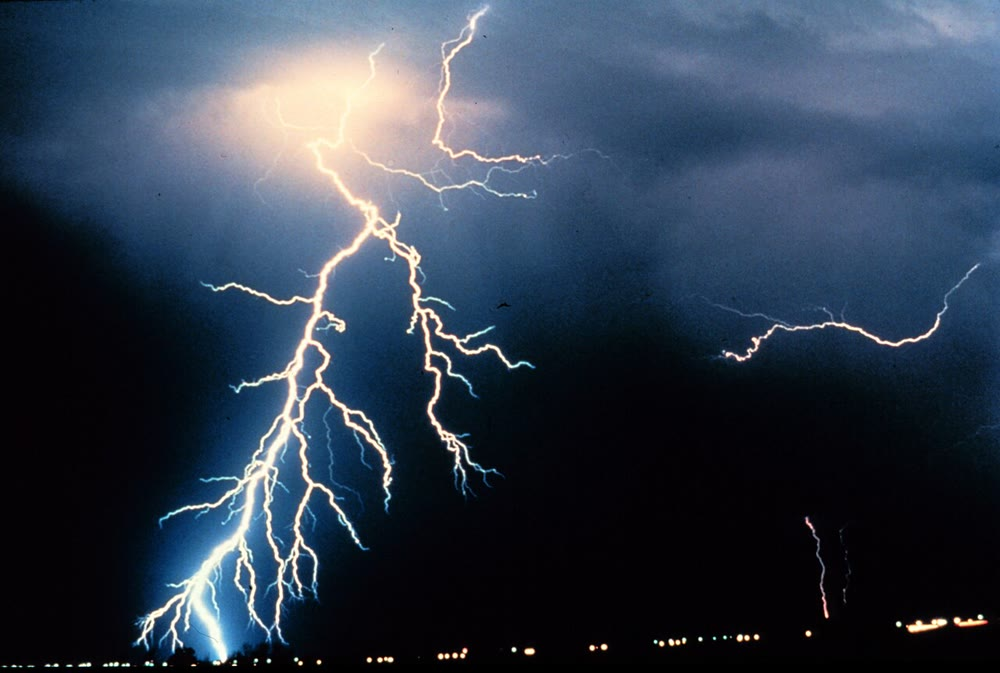
\includegraphics[width=0.62\linewidth]{images/book2/g10-noaa-lightning.jpg}

{\small Sambaran \omterm{def:g10:storms-and-cyclones:lightning}{petir}, di antara awan dan dari awan ke tanah, selama \omterm{def:g10:storms-and-cyclones:thunderstorm}{badai
guntur} pada malam hari. Foto: C.~Clark, NOAA National Severe Storms Laboratory
(domain publik).}
\end{omfigure}

Satelit yang menghitung kilatan cahaya di seluruh planet mendapati sekitar
1.4 miliar kilatan \omterm{def:g10:storms-and-cyclones:lightning}{petir} setahun, atau 44 setiap detik.
% ledger: christian:flash-rate

\begin{method}[Jarak badai dari kilatan sampai guntur]\label{met:g10:storms-and-cyclones:distance}
\begin{enumerate}
  \item Cahaya kilatan tiba praktis seketika; guntur merambat dengan laju
        bunyi, sekitar \qty{343}{m/s} pada \qty{20}{\degreeCelsius}.
  \item Hitung detik $t$ di antara kilatan dan guntur.
  \item Jaraknya $343\,t$ meter: sekitar \qty{1}{km} untuk setiap
        tiga detik.
\end{enumerate}
\end{method}
% ledger: const:R, earth:Mmol (speed of sound computed in figdata/grade-10/cyclones.py)

\section{Tornado}

\begin{definition}[Tornado]\label{def:g10:storms-and-cyclones:tornado}
Yang disebut \emph{tornado}\index{tornado} adalah kolom udara yang berputar
dengan dahsyat dan bersentuhan dengan tanah, menggantung dari dasar sebuah
kumulonimbus.
\end{definition}

\omterm{def:g10:storms-and-cyclones:tornado}{Tornado} terkuat berasal dari \emph{superkel}, yaitu \omterm{def:g10:storms-and-cyclones:thunderstorm}{badai guntur} yang arus
naiknya berputar secara keseluruhan. \omterm{def:g10:storms-and-cyclones:tornado}{Tornado} kecil dan singkat: biasanya
lebarnya beberapa ratus meter, berlangsung beberapa menit, dengan lintasan
rata-rata sekitar \qty{5.6}{km}. Namun anginnya adalah yang terkuat di
permukaan Bumi: sebuah radar bergerak mengukur sekitar \qty{135}{m/s} (sekitar
\qty{480}{km/h}) di atas tanah dalam sebuah \omterm{def:g10:storms-and-cyclones:tornado}{tornado} di Oklahoma pada Mei 1999.
Amerika Serikat mengalami lebih banyak \omterm{def:g10:storms-and-cyclones:tornado}{tornado} daripada negara lain mana pun,
sekitar 1200 setahun; daerah lain tempat \omterm{def:g10:storms-and-cyclones:tornado}{tornado} sering terjadi antara lain
padang rumput Kanada, Bangladesh, Argentina utara dan Brasil selatan, serta
Britania Raya.
% ledger: spc:tornado

\begin{omfigure}
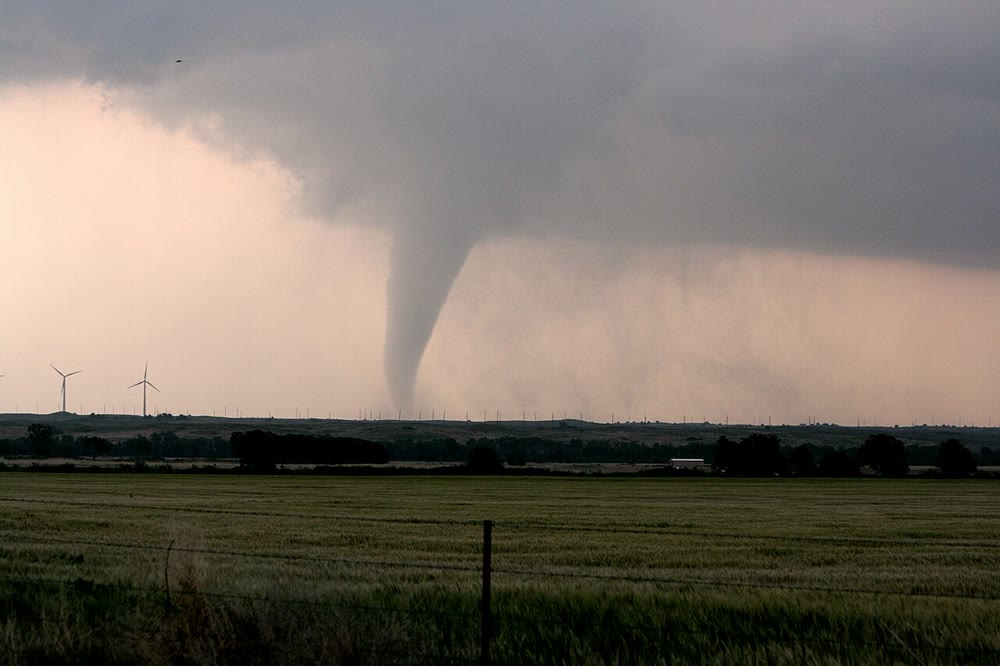
\includegraphics[width=0.62\linewidth]{images/book2/g10-noaa-tornado-kansas.jpg}

{\small Sebuah \omterm{def:g10:storms-and-cyclones:tornado}{tornado} di atas dataran Kansas, Mei 2008: corongnya menggantung
dari dasar awan badai. Foto: Sean Waugh, NOAA National Severe Storms
Laboratory (domain publik).}
\end{omfigure}

\section{Siklon tropis}

\begin{definition}[Siklon tropis; mata; dinding mata]\label{def:g10:storms-and-cyclones:tropical-cyclone}
Yang disebut \emph{siklon tropis}\index{siklon tropis} adalah badai yang
lebarnya ratusan kilometer, yang terbentuk di atas laut tropis yang hangat di
sekitar pusat bertekanan rendah, dengan angin yang berpilin masuk ke arah
pusat dan pita-pita \omterm{def:g10:storms-and-cyclones:thunderstorm}{badai guntur}. Bila angin tetapnya mencapai \num{64}~knot,
sekitar \qty{119}{km/h}, siklon itu disebut hurikan di Atlantik dan Pasifik
timur, taifun di Pasifik barat, dan cukup siklon di Samudra Hindia dan Pasifik
Selatan. Pusatnya yang tenang dan hampir tanpa awan adalah
\emph{mata}\index{mata (siklon)}; cincin \omterm{def:g10:storms-and-cyclones:thunderstorm}{badai guntur} yang menjulang di
sekelilingnya, tempat angin paling kuat, adalah \emph{dinding
mata}\index{dinding mata}.
\end{definition}
% ledger: nhc:sshws

\begin{omfigure}
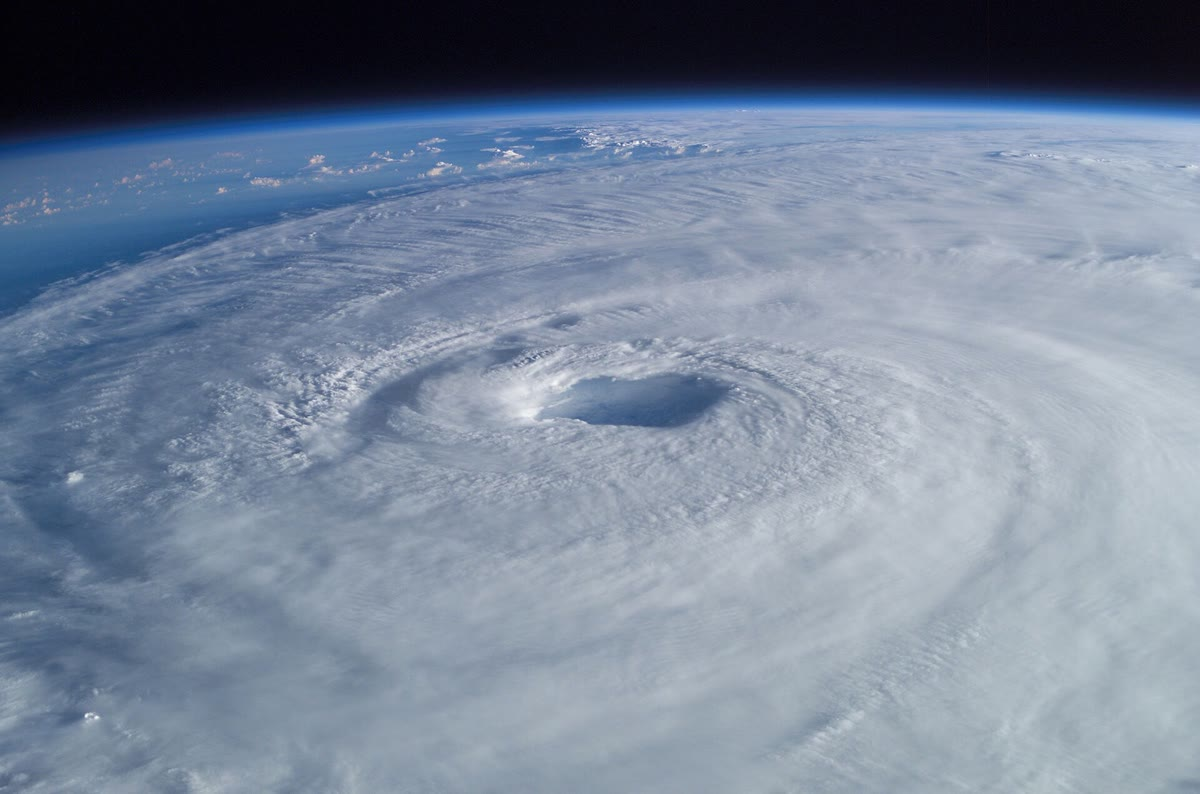
\includegraphics[width=0.78\linewidth]{images/book2/g10-nasa-hurricane-isabel.jpg}

{\small Hurikan Isabel, 15 September 2003, difoto oleh seorang astronaut dari
Stasiun Antariksa Internasional: \omterm{def:g10:storms-and-cyclones:tropical-cyclone}{mata}, \omterm{def:g10:storms-and-cyclones:tropical-cyclone}{dinding mata}, dan pilinan awan di
sekelilingnya. Citra: Mike Trenchard, Earth Sciences and Image Analysis
Laboratory, NASA Johnson Space Center (domain publik).}
\end{omfigure}

Di dekat permukaan laut, udara lembap mengalir masuk ke arah tekanan rendah di
pusat. Rotasi Bumi membelokkan udara yang bergerak ke kanan di belahan bumi
utara: alih-alih langsung menuju pusat, udara itu berputar mengelilinginya,
berlawanan arah jarum jam bila dilihat dari atas (searah jarum jam di belahan
bumi selatan). Di dekat pusat udara itu naik di \omterm{def:g10:storms-and-cyclones:tropical-cyclone}{dinding mata}, mengembun, dan
mengalir keluar di puncak badai. Di dalam \omterm{def:g10:storms-and-cyclones:tropical-cyclone}{mata}, sedikit udara turun,
menghangat, dan mengering: langit menjadi cerah.

\begin{omfigure}
\begin{tikzpicture}[font=\footnotesize, >={Stealth[length=2mm]}]
  \fill[omDef!25] (-6,-0.4) rectangle (6,0);
  \node[anchor=north, omDef!80!black] at (0,-0.05) {laut hangat};
  % rain bands
  \foreach \x/\h in {-5.0/1.6, -3.9/2.2, 3.9/2.2, 5.0/1.6}
    \fill[black!10, draw=black!45] (\x-0.35,0.4) -- (\x-0.3,\h) .. controls (\x-0.15,\h+0.35) and (\x+0.15,\h+0.35) .. (\x+0.3,\h) -- (\x+0.35,0.4) -- cycle;
  % eyewall towers and outflow canopy
  \fill[black!14, draw=black!50] (-2.4,0.4) -- (-2.5,4.0) -- (-5.8,4.3) -- (-5.6,4.7) -- (-1.0,4.9) -- (-0.75,4.0) -- (-0.8,0.4) -- cycle;
  \fill[black!14, draw=black!50] (2.4,0.4) -- (2.5,4.0) -- (5.8,4.3) -- (5.6,4.7) -- (1.0,4.9) -- (0.75,4.0) -- (0.8,0.4) -- cycle;
  % inflow, rise, outflow, eye subsidence
  \draw[->, thick, omThm!80!black] (-5.8,0.2) -- (-1.3,0.2) -- (-1.3,4.3) -- (-4.2,4.45);
  \draw[->, thick, omThm!80!black] (5.8,0.2) -- (1.3,0.2) -- (1.3,4.3) -- (4.2,4.45);
  \draw[->, thick, omDef!80!black] (0,4.3) -- (0,1.0);
  \node[anchor=south, align=center] at (0,5.0) {mata: udara kering\\yang turun};
  \node[anchor=south east, align=right] at (-2.6,4.95) {dinding mata};
  \node[anchor=west, align=left] at (-5.95,2.9) {pita\\hujan};
  \node[anchor=north, align=center] at (-3.6,0.15) {aliran masuk lembap};
  \node[anchor=south east, align=right] at (5.8,4.95) {aliran keluar di atas};
  % plan view
  \begin{scope}[shift={(8.4,2.3)}]
    \draw[black!40] (0,0) circle (1.7);
    \foreach \a in {0,90,180,270}
      \draw[->, thick, omThm!80!black, domain=0:200, samples=30, variable=\t]
        plot ({(1.6-0.0045*\t)*cos(\a+\t)}, {(1.6-0.0045*\t)*sin(\a+\t)});
    \fill[white, draw=black!50] (0,0) circle (0.22);
    \node[anchor=north, align=center] at (0,-1.8) {dilihat dari atas\\(belahan bumi utara)};
  \end{scope}
\end{tikzpicture}

{\small \omterm{def:g10:storms-and-cyclones:tropical-cyclone}{Siklon tropis} dalam penampang (skematis, ketinggian sangat
dibesar-besarkan): udara lembap mengalir masuk di atas laut yang hangat, naik
di \omterm{def:g10:storms-and-cyclones:tropical-cyclone}{dinding mata} dan pita-pita hujan, lalu mengalir keluar di puncak; sedikit
udara turun di dalam \omterm{def:g10:storms-and-cyclones:tropical-cyclone}{mata}. Kanan: dilihat dari atas di belahan bumi utara,
aliran masuk berputar berlawanan arah jarum jam mengelilingi pusat.}
\end{omfigure}

\omterm{def:g10:storms-and-cyclones:tropical-cyclone}{Siklon tropis} memerlukan samudra yang hangat: air bersuhu sekurang-kurangnya
sekitar \qty{27}{\degreeCelsius} di permukaan, yang hangat sampai kedalaman
sekitar \qty{46}{m}. \omterm{def:g10:storms-and-cyclones:tropical-cyclone}{Siklon tropis} tidak terbentuk tepat di khatulistiwa,
tempat rotasi Bumi tidak membelokkan udara yang mengalir masuk: sebuah badai
harus berada sekurang-kurangnya sekitar \qty{480}{km} dari khatulistiwa agar
putarannya dapat dimulai.
% ledger: aoml:formation

\begin{omfigure}
\begin{tikzpicture}
\begin{axis}[ommap, width=\linewidth, xtick={-180,-120,...,180}, ytick={-60,-30,0,30,60},
  ymin=-70, ymax=70, unbounded coords=jump]
\addplot[fill=omLithAlluv, draw=black!45, line width=0.2pt] table {figdata/out/shared-geo-land.dat};
\addplot[omThm!70, line width=0.25pt] table {figdata/out/grade-10-cyclones-tracks.dat};
\addplot[only marks, mark=*, mark size=0.45pt, omDef!90!black] table {figdata/out/grade-10-cyclones-genesis.dat};
\addplot[black!45, dashed, domain=-180:180] {0};
\end{axis}
\end{tikzpicture}

{\small \omterm{def:g10:storms-and-cyclones:tropical-cyclone}{Siklon tropis}: lintasan semua badai pada musim 2015--2024 (merah), dan
tempat setiap badai pada musim 1980--2024 pertama kali mencapai kekuatan badai
tropis (titik biru). Data: IBTrACS v04r01, NOAA National Centers for
Environmental Information.}
\end{omfigure}
% ledger: data:b2-ibtracs (all statistics computed in figdata/grade-10/cyclones.py)

Peta itu memperlihatkan aturan tersebut. Dari 3\,888 badai pada 1980--2024,
hanya 24 yang mencapai kekuatan badai tropis dalam jarak \qty{5}{\degree} dari
khatulistiwa. Sebagian besar terbentuk di antara lintang \qty{10}{\degree} dan
\qty{30}{\degree}, lalu hanyut ke barat bersama angin pasat dan membelok
menjauh ke arah kutub, tempat laut yang dingin melemahkannya. Atlantik
Selatan, yang lebih sejuk dan kurang mendukung, hanya mengalami tiga dalam 45
tahun. Sekitar 87 \omterm{def:g10:storms-and-cyclones:tropical-cyclone}{siklon tropis} terbentuk dalam setahun rata-rata, tujuh dari
sepuluh di antaranya di belahan bumi utara, dan sedikit lebih dari separuhnya
mencapai kekuatan hurikan.

\begin{proposition}[Sumber energi siklon tropis]\label{prop:g10:storms-and-cyclones:energy}
\omterm{def:g10:storms-and-cyclones:tropical-cyclone}{Siklon tropis} mengambil energinya dari laut yang hangat: \omterm{def:g10:earth-energy-budget:latent-heat}{kalor laten} yang
diserap oleh penguapan di permukaan laut dilepaskan di \omterm{def:g10:storms-and-cyclones:tropical-cyclone}{dinding mata} dan
pita-pita hujan ketika uap mengembun. Hurikan rata-rata melepaskan dengan cara
ini sekitar \qty{6e14}{W}; hanya sebagian kecil darinya, sekitar
\qty{1.5e12}{W}, menjadi energi kinetik anginnya.
\end{proposition}
% ledger: aoml:energy

\begin{proof}[Pembenaran]
Hurikan rata-rata menurunkan hujan \qty{1.5}{cm} sehari di atas lingkaran
berjari-jari \qty{665}{km}, dengan luas $\pi \times (665\,000)^2 \approx
\qty{1.39e12}{m^2}$: \qty{2.1e10}{m^3}, atau \qty{2.1e13}{kg}, air sehari.
Setiap kilogram yang mengembun melepaskan sekitar \qty{2.5}{MJ}: $2.1\times10^{13}
\times 2.5\times10^6 \approx \qty{5.2e19}{J}$ sehari, yaitu
$5.2\times10^{19}/86\,400 \approx \qty{6.0e14}{W}$. Daya angin adalah
perkiraan dari medan angin yang terukur, dikutip dari sumber yang sama.
\end{proof}

Badai itu bekerja seperti mesin: kalor diterima di permukaan laut yang hangat,
dilepaskan tinggi di udara atas yang dingin, dan sebagian selisihnya diubah
menjadi gerak angin. Itulah sebabnya \omterm{def:g10:storms-and-cyclones:tropical-cyclone}{siklon tropis} cepat melemah ketika
bergerak ke atas daratan atau ke atas air yang dingin: siklon itu kehilangan
pasokan air yang menguap.

\section{Intensitas, angin, dan gelombang badai}

\begin{definition}[Skala Saffir--Simpson]\label{def:g10:storms-and-cyclones:scale}
Yang disebut \emph{skala Saffir--Simpson}\index{skala Saffir--Simpson} adalah
skala yang memilah hurikan ke dalam lima kategori menurut angin tetap
maksimumnya; kategori 3 sampai 5 adalah hurikan \emph{besar}.
\end{definition}

\begin{center}
\small
\begin{tabular}{cccc}
\hline
kategori & knot & \unit{m/s} & \unit{km/h} \\
\hline
1 & 64--82 & 33--42 & 119--153 \\
2 & 83--95 & 43--49 & 154--177 \\
3 & 96--112 & 49--58 & 178--208 \\
4 & 113--136 & 58--70 & 209--251 \\
5 & 137 atau lebih & 70 atau lebih & 252 atau lebih \\
\hline
\end{tabular}
\end{center}
% ledger: nhc:sshws (m/s converted with 1 knot = 1852/3600 m/s)

Makin dalam tekanan rendah di pusat, makin kuat angin yang bertiup
mengelilinginya: selisih tekanan antara pusat dan sekitarnya itulah yang
mendorong udara ke dalam.

\begin{omfigure}
\begin{tikzpicture}
\begin{axis}[omrecord, width=0.86\linewidth, height=6.2cm, xmin=15, xmax=100,
  ymin=860, ymax=1015, xlabel={angin tetap maksimum (\unit{m/s})},
  ylabel={tekanan pusat minimum (\unit{hPa})},
  tick label style={font=\small}, label style={font=\small}]
\foreach \w in {32.92, 42.70, 49.39, 58.13, 70.48}
  \edef\temp{\noexpand\draw[black!55, densely dashed] (axis cs:\w,860) -- (axis cs:\w,1015);}\temp
\addplot[only marks, mark=*, mark size=0.6pt, omDef!80!black, opacity=0.6] table[x=wind_ms, y=pmin_hpa] {figdata/out/grade-10-cyclones-scatter.dat};
\addplot[omThm!85!black, thick] table[x=wind_ms, y=pmin_hpa] {figdata/out/grade-10-cyclones-fit.dat};
\node[font=\scriptsize, black!60] at (axis cs:37.8,1008) {1};
\node[font=\scriptsize, black!60] at (axis cs:46.0,1008) {2};
\node[font=\scriptsize, black!60] at (axis cs:53.8,1008) {3};
\node[font=\scriptsize, black!60] at (axis cs:64.3,1008) {4};
\node[font=\scriptsize, black!60] at (axis cs:76,1008) {5};
\end{axis}
\end{tikzpicture}

{\small Setiap titik adalah satu \omterm{def:g10:storms-and-cyclones:tropical-cyclone}{siklon tropis} pada musim 2000--2024: angin
tetapnya yang terkuat dan tekanan pusatnya yang terendah. Garisnya adalah
garis lurus yang paling cocok: sekitar \qty{1.6}{hPa} lebih rendah untuk
setiap tambahan satu meter per detik. Garis putus-putus kelabu: batas-batas
kategori Saffir--Simpson (bernomor di bagian atas). Data: IBTrACS v04r01, NOAA
NCEI.}
\end{omfigure}
% ledger: data:b2-ibtracs, nhc:sshws (fit computed in figdata/grade-10/cyclones.py)

Rekor badai 1980--2024 dalam arsip itu dipegang oleh Hurikan Patricia, di
lepas pantai Pasifik Meksiko pada Oktober 2015: angin tetap 185 knot, sekitar
\qty{95}{m/s}, dan tekanan pusat \qty{872}{hPa}.
% ledger: data:b2-ibtracs

\begin{definition}[Gelombang badai]\label{def:g10:storms-and-cyclones:storm-surge}
Yang disebut \emph{gelombang badai}\index{gelombang badai} adalah kenaikan
muka laut di atas aras normalnya, tidak termasuk pasang surut, yang disebabkan
oleh badai: angin menumpuk air ke arah pesisir, dan tekanan rendah membuat
laut menggembung di bawah badai.
\end{definition}

\begin{proposition}[Gembungan tekanan]\label{prop:g10:storms-and-cyclones:bulge}
Di bawah badai yang tekanan pusatnya $\Delta p$ hektopascal di bawah tekanan
sekitarnya, laut naik sekitar $\Delta p$ sentimeter.
\end{proposition}

\begin{proof}
Jauh di bawah permukaan, tekanan harus sama di bawah badai dan di luarnya;
jika tidak, air akan mengalir. Udara di atas badai lebih ringan sebesar
$\Delta p$; kolom air laut setinggi $h$ mengimbanginya jika
$\rho g h = \Delta p$. Untuk $\Delta p = \qty{1}{hPa} = \qty{100}{Pa}$, dengan
$\rho = \qty{1025}{kg/m^3}$ dan $g = \qty{9.81}{m/s^2}$: $h = 100/(1025
\times 9.81) \approx \qty{0.0099}{m}$, sekitar \qty{1}{cm}.
\end{proof}
% ledger: noaa:seawater-1025, nasa:aquarius-density, const:gn

Gembungan itu adalah bagian yang lebih kecil dari sebagian besar \omterm{def:g10:storms-and-cyclones:storm-surge}{gelombang
badai}: di bawah tekanan pusat \qty{920}{hPa}, \qty{90}{hPa} di bawah
sekitarnya, gembungan itu sekitar \qty{0.9}{m}. Angin melakukan sisanya,
mendorong air ke arah pantai, terutama di atas dasar laut yang lebar dan
dangkal. Bila datang bersamaan dengan pasang naik, \omterm{def:g10:storms-and-cyclones:storm-surge}{gelombang badai} setinggi
beberapa meter dapat membanjiri pesisir yang rendah sampai jauh ke pedalaman.

\begin{omfigure}
\begin{tikzpicture}[font=\footnotesize, >={Stealth[length=2mm]}]
  \def\surf{(0,0) .. controls (1.5,0) and (2.2,0.5) .. (3.0,0.5) .. controls (3.8,0.5) and (4.6,0.4) .. (5.6,0.5) .. controls (7.2,0.65) and (8.8,1.0) .. (10.25,1.3)}
  \fill[omDef!20] (0,-1.6) -- \surf -- (8.8,-1.6) -- cycle;
  \draw[thick, omDef!80!black] \surf;
  \draw[black!50, dashed] (0,0) -- (9.6,0);
  \node[anchor=north west, black!60] at (0.1,-0.05) {muka laut normal};
  \fill[omExo!30, draw=black!60] (8.8,-1.6) -- (10.4,1.6) -- (12.4,1.7) -- (12.4,-1.6) -- cycle;
  \foreach \x in {10.9,11.7} \draw[fill=white, draw=black!60] (\x,1.63) rectangle (\x+0.45,2.03) (\x-0.05,2.03) -- (\x+0.225,2.28) -- (\x+0.5,2.03);
  \draw[<->, omThm!80!black] (3.0,0) -- (3.0,0.5);
  \node[anchor=south east, omThm!80!black, align=right] at (2.8,0.6) {gembungan di bawah\\tekanan rendah};
  \draw[<->, omThm!80!black] (9.4,0) -- (9.4,1.12);
  \node[anchor=south, omThm!80!black, align=center] at (8.9,1.75) {penumpukan oleh angin\\di pesisir};
  \foreach \y in {2.9,3.4} \draw[->, thick, black!60] (4.0,\y) -- (6.4,\y);
  \node[anchor=south] at (5.2,3.45) {angin ke darat};
  \node[anchor=south, align=center] at (3.0,1.9) {pusat\\badai};
  \draw[black!40] (3.0,1.9) -- (3.0,0.65);
\end{tikzpicture}

{\small \omterm{def:g10:storms-and-cyclones:storm-surge}{Gelombang badai} (skematis, ketinggian sangat dibesar-besarkan): laut
naik sekitar \qty{1}{cm} untuk setiap hektopascal tekanan rendah di bawah
badai, dan angin ke darat menumpuk air ke arah pesisir.}
\end{omfigure}

\begin{omfigure}
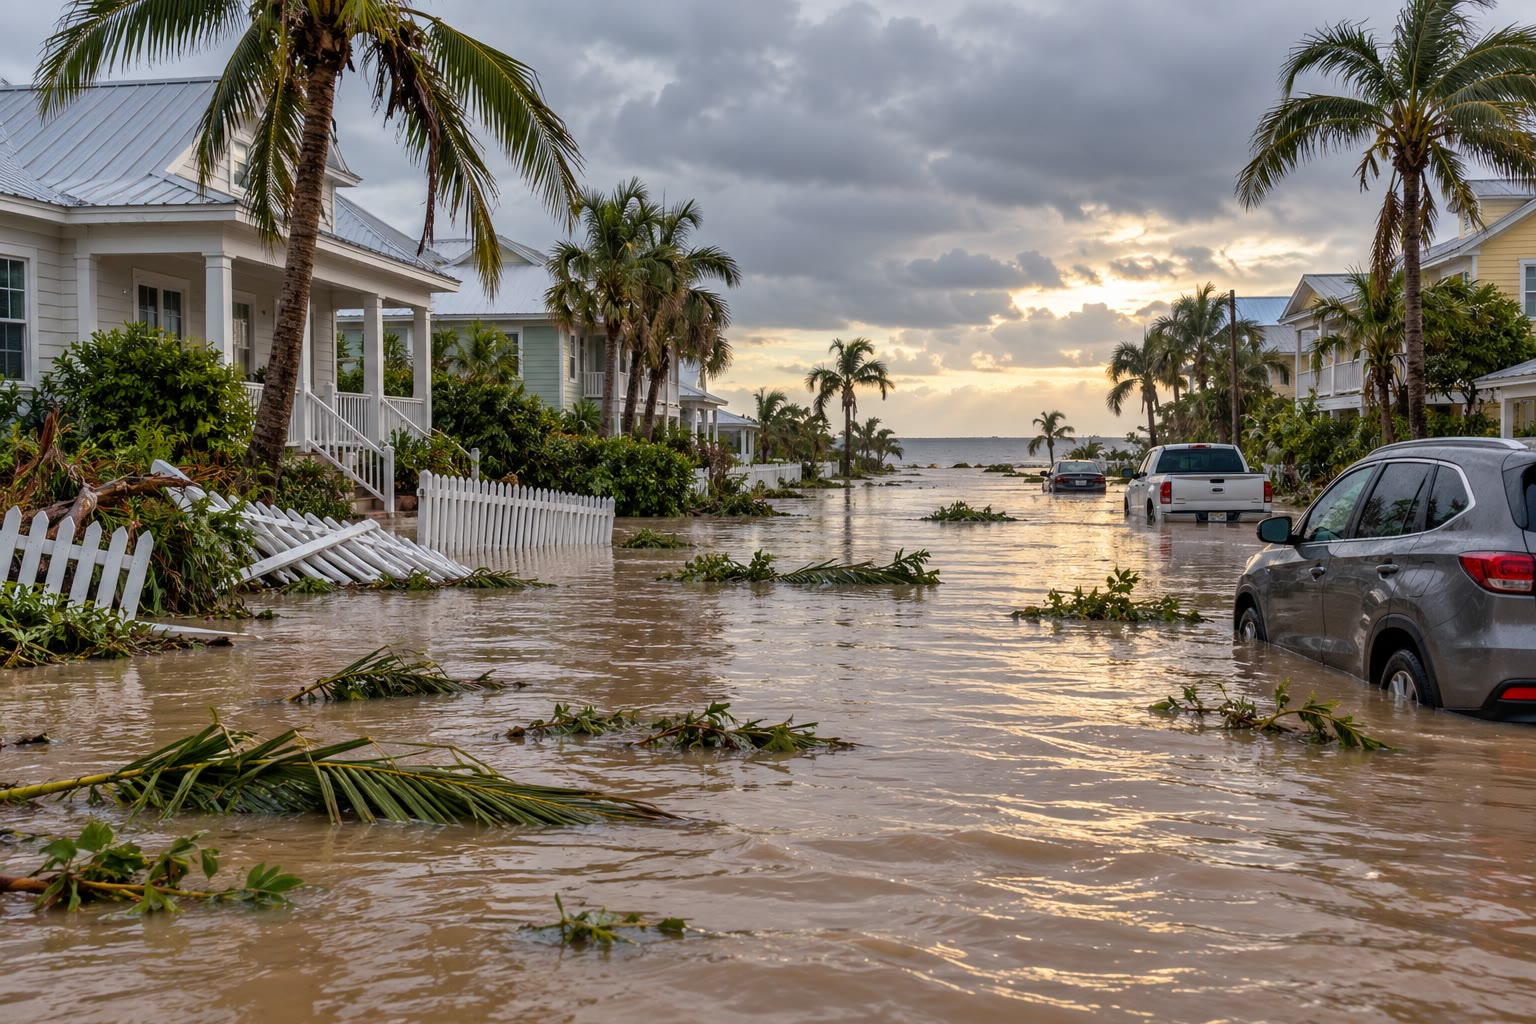
\includegraphics[width=0.7\linewidth]{images/book2/ai/g10-flooded-street.jpg}

{\small Sebuah jalan di pesisir pada pagi hari setelah \omterm{def:g10:storms-and-cyclones:storm-surge}{gelombang badai}: air
laut, pohon palem yang patah, dan pagar yang robek.}
\end{omfigure}

\section{Latihan}

\begin{exercise}[$\star$]\label{exo:g10:storms-and-cyclones:1}
Definisikan \omterm{def:g10:storms-and-cyclones:thunderstorm}{badai guntur} dan \omterm{def:g10:storms-and-cyclones:lightning}{petir}. Apa yang menghasilkan bunyi guntur?
\end{exercise}

\begin{exercise}[$\star$]\label{exo:g10:storms-and-cyclones:2}
Definisikan \omterm{def:g10:storms-and-cyclones:tropical-cyclone}{siklon tropis}, \omterm{def:g10:storms-and-cyclones:tropical-cyclone}{matanya}, dan \omterm{def:g10:storms-and-cyclones:tropical-cyclone}{dinding matanya}. Di manakah anginnya
paling kuat?
\end{exercise}

\begin{exercise}[$\star$]\label{exo:g10:storms-and-cyclones:3}
Dalam kategori Saffir--Simpson manakah hurikan dengan angin tetap
\num{70}~knot? \num{120}~knot? \num{140}~knot? Manakah di antaranya yang
merupakan hurikan besar?
\end{exercise}

\begin{exercise}[$\star$]\label{exo:g10:storms-and-cyclones:4}
Kamu menghitung \num{9} detik di antara sebuah kilatan dan gunturnya, lalu
\num{15} detik untuk kilatan berikutnya. Berapa jauh masing-masing, dan apakah
badai itu mendekat?
\end{exercise}

\begin{exercise}[$\star$]\label{exo:g10:storms-and-cyclones:5}
Jelaskan mengapa pohon yang berdiri sendirian di lapangan adalah tempat
berlindung yang berbahaya saat \omterm{def:g10:storms-and-cyclones:thunderstorm}{badai guntur}, dan ke mana kamu seharusnya
pergi.
\end{exercise}

\begin{exercise}[$\star\star$]\label{exo:g10:storms-and-cyclones:6}
Satu knot adalah \qty{1852}{m} per jam. Ubahlah \num{64}~knot dan
\num{137}~knot ke dalam \unit{m/s} dan \unit{km/h}.
\end{exercise}

\begin{exercise}[$\star\star$]\label{exo:g10:storms-and-cyclones:7}
Ada 44 kilatan \omterm{def:g10:storms-and-cyclones:lightning}{petir} setiap detik di Bumi. Berapa banyak itu dalam sehari,
dan dalam setahun?
\end{exercise}

\begin{exercise}[$\star\star$]\label{exo:g10:storms-and-cyclones:8}
Sebuah hurikan memiliki tekanan pusat \qty{935}{hPa} dengan tekanan sekitar
\qty{1010}{hPa}. Berapa tinggi gembungan tekanan laut di bawahnya?
\end{exercise}

\begin{exercise}[$\star\star$]\label{exo:g10:storms-and-cyclones:9}
Dengan peta lintasan, uraikan di mana \omterm{def:g10:storms-and-cyclones:tropical-cyclone}{siklon tropis} terbentuk dan ke mana
siklon itu pergi setelah terbentuk. Mengapa \omterm{def:g10:storms-and-cyclones:tropical-cyclone}{siklon tropis} tidak ada tepat di
khatulistiwa?
\end{exercise}

\begin{exercise}[$\star\star$]\label{exo:g10:storms-and-cyclones:10}
Garis lurus pada grafik tekanan--angin adalah $p \approx 1031 - 1.56\,v$
($p$ dalam \unit{hPa}, $v$ dalam \unit{m/s}). Berapa tekanan pusat yang
diberikannya untuk batas bawah kategori 5, \qty{70}{m/s}? Untuk badai
\qty{40}{m/s}?
\end{exercise}

\begin{exercise}[$\star\star$]\label{exo:g10:storms-and-cyclones:11}
Jelaskan mengapa \omterm{def:g10:storms-and-cyclones:tropical-cyclone}{siklon tropis} cepat melemah ketika bergerak ke atas daratan,
dan mengapa siklon itu melemah di atas air yang dingin.
\end{exercise}

\begin{exercise}[$\star\star\star$]\label{exo:g10:storms-and-cyclones:12}
Laju bunyi di udara adalah $\sqrt{1.4\,R\,T/M}$, dengan $R =
\qty{8.314}{J.mol^{-1}.K^{-1}}$, $T$ dalam kelvin, dan $M =
\qty{0.02897}{kg/mol}$. Hitung laju itu pada \qty{0}{\degreeCelsius} dan pada
\qty{30}{\degreeCelsius}. Untuk selang waktu \qty{9}{s}, berapa selisih kedua
jaraknya? Apakah aturan ``\qty{3}{s} per kilometer'' cukup baik?
\end{exercise}

\begin{exercise}[$\star\star\star$]\label{exo:g10:storms-and-cyclones:13}
\omterm{def:g10:storms-and-cyclones:storm-surge}{Gelombang badai} setinggi \qty{4.0}{m} terukur di sebuah pesisir ketika hurikan
dengan tekanan pusat \qty{940}{hPa} (tekanan sekitar \qty{1010}{hPa}) mendarat.
Berapa bagian dari gelombang itu yang disebabkan oleh gembungan tekanan, dan
berapa oleh angin? Jika gelombang itu datang saat pasang naik, \qty{1.5}{m} di
atas muka laut rata-rata, setinggi apa air mencapai di atas muka laut
rata-rata?
\end{exercise}

\begin{exercise}[$\star\star\star$]\label{exo:g10:storms-and-cyclones:14}
Sebuah \omterm{def:g10:storms-and-cyclones:tornado}{tornado} berputar dengan angin \qty{90}{m/s} pada jarak \qty{100}{m}
dari sumbunya; sebuah hurikan dengan angin \qty{60}{m/s} di \omterm{def:g10:storms-and-cyclones:tropical-cyclone}{dinding mata}
\qty{30}{km} dari pusat. Berapa lama udara memerlukan waktu untuk berputar satu
kali dalam masing-masing kasus? Bandingkan.
\end{exercise}

\begin{exercise}[$\star\star\star$]\label{exo:g10:storms-and-cyclones:15}
Dari 3\,888 \omterm{def:g10:storms-and-cyclones:tropical-cyclone}{siklon tropis} pada 1980--2024, 24 mencapai kekuatan badai tropis
dalam jarak \qty{5}{\degree} dari khatulistiwa, 414 dalam jarak
\qty{10}{\degree}, dan 121 di luar \qty{30}{\degree}. Hitung ketiga
persentasenya. Pita selebar \qty{5}{\degree} di kedua sisi khatulistiwa
meliputi sekitar \qty{9}{\percent} permukaan Bumi: apa yang akan kamu harapkan
jika lintang tidak berpengaruh, dan apa kesimpulanmu?
\end{exercise}

\section{Soal: Mesin Kalor Sebuah Hurikan}

\begin{problem}[{Soal akhir pekan --- dari hujan sehari sampai daya
angin}]
\label{pb:g10:storms-and-cyclones:1}
% ledger: aoml:energy, nist:water-latent, earth:Rmean, ipcc:budget-toa (all results computed in figdata/grade-10/cyclones.py or from the rounded data below)
Hurikan rata-rata menurunkan hujan \qty{1.5}{cm} sehari di atas lingkaran
berjari-jari \qty{665}{km}. Gunakan \omterm{def:g10:earth-energy-budget:latent-heat}{kalor laten} \qty{2.5}{MJ/kg}, massa jenis
air \qty{1000}{kg/m^3}, \qty{86400}{s} dalam sehari, dan daya angin hurikan
rata-rata, \qty{1.5e12}{W}.

\medskip
\noindent\textbf{Bagian I --- Hujan sehari.}
\begin{enumerate}
  \item Hitung luas lingkaran itu.
  \item Hitung volume hujan yang jatuh di atasnya dalam sehari.
  \item Nyatakan volume itu dalam kilometer kubik.
  \item Hitung massanya.
\end{enumerate}

\medskip
\noindent\textbf{Bagian II --- Kalor yang dilepaskan.}
\begin{enumerate}[resume]
  \item Hitung \omterm{def:g10:earth-energy-budget:latent-heat}{kalor laten} yang dilepaskan dalam sehari oleh pengembunan
        air ini.
  \item Ubahlah kalor itu menjadi daya.
  \item Seluruh Bumi menyerap sekitar \qty{1.22e17}{W} cahaya Matahari
        (\cref{ch:g10:earth-energy-budget}). Berapa bagian darinya yang
        dilepaskan oleh satu hurikan?
  \item Cahaya Matahari rata-rata yang diserap adalah \qty{240}{W/m^2}.
        Hitung cahaya Matahari yang diserap oleh luas badai itu dan
        bandingkan dengan \omterm{def:g10:earth-energy-budget:latent-heat}{kalor laten} badai itu.
  \item Apa yang diperlihatkan perbandingan ini tentang tempat energi badai
        itu dikumpulkan?
\end{enumerate}

\medskip
\noindent\textbf{Bagian III --- Dari mana airnya berasal.}
\begin{enumerate}[resume]
  \item Berapa massa air yang harus menguap setiap hari untuk memasok hujan
        ini?
  \item Penguapan rata-rata permukaan Bumi membawa \qty{82}{W/m^2}. Di atas
        luas berapa penguapan rata-rata akan memasok \omterm{def:g10:earth-energy-budget:latent-heat}{kalor laten} badai itu?
        Bandingkan dengan luas badai.
  \item Dengan tabel kandungan jenuh pada \cref{ch:g10:why-clouds-form},
        bandingkan air yang ditampung udara jenuh pada
        \qty{28}{\degreeCelsius} dan pada \qty{20}{\degreeCelsius}.
  \item Jelaskan mengapa \omterm{def:g10:storms-and-cyclones:tropical-cyclone}{siklon tropis} hanya terbentuk di atas laut yang
        hangat.
  \item Jelaskan mengapa \omterm{def:g10:storms-and-cyclones:tropical-cyclone}{siklon tropis} melemah di atas daratan.
\end{enumerate}

\medskip
\noindent\textbf{Bagian IV --- Angin.}
\begin{enumerate}[resume]
  \item Hitung energi kinetik yang diberikan kepada angin dalam sehari.
  \item Ubahlah batas bawah kategori 3, \num{96}~knot, ke dalam
        \unit{m/s} (\num{1}~knot = \qty{1852}{m/h}).
  \item Udara di dekat permukaan laut memiliki massa jenis sekitar
        \qty{1.16}{kg/m^3}. Hitung energi kinetik satu meter kubik udara
        itu yang bergerak dengan laju tersebut.
  \item Bandingkan \omterm{def:g10:earth-energy-budget:latent-heat}{kalor laten} yang dilepaskan dalam sehari dengan energi
        angin dalam sehari.
  \item Apa yang terjadi dengan sisa kalor yang dilepaskan?
  \item Berapa bagian kalor yang dilepaskan oleh pengembunan yang menjadi
        angin?
\end{enumerate}
\end{problem}
